\chapter{General Concepts in Adversarial Distributed Systems}

% \subimport{./}{flp-impossibility.tex}

\subimport{./}{pos-and-nothing-at-stake.tex}

\subimport{./}{wealth-inequality.tex}

\subimport{./}{mev.tex}

\section{The ever growing state, state expiry}
State expiry refers to removing state from individual nodes if it hasn't been accessed recently. There are several ways this could be implemented, including:

\textbf{Expire by rent}: charging "rent" to accounts and expiring them when their rent reaches zero. This design is implemented in Solana.

\textbf{Expire by time}: making accounts inactive if there are no reading/writing to that account for some amount of time


\section{Rebuilding the chain / Chain Derivation}

\section{Supporting a different virtual machine}
Execution of code in any blockchain assumes an "execution environment". This execution environment is often called the "virtual machine" that blockchain is running. For example, Ethereum runs the EVM, the \textbf{E}thereum \textbf{V}irtual \textbf{M}achine. Solana runs the SVM similarly.

A curious question arises: \textbf{Can a virtual machine non-native to a blockchain be introduced as a co-execution environment?}. The answer to this is a resounding yes. However, one needs to question the intent of doing this. Almost all execution environments are \href{https://www.bitstamp.net/learn/blockchain/what-is-turing-complete/}{turing complete}, however the cost of executions may be prohibitive at times.

One such use-case is extending the EVM with capabilities to run WASM or RISC-V code. A couple interesting projects doing this would be \href{https://arbitrum.io/stylus}{Arbitrum Stylus} and \href{https://hackmd.io/@leoalt/r55}{R55}.

\subsubsection{Arbitrum Stylus}
Stylus extends the execution environment to run WASM-targeted smart contracts. Instead of writing in solidity, one writes the code in languages like Rust, Zig, Go, Sway, Swift. Rust is supported as primary language and \href{https://docs.arbitrum.io/stylus/reference/overview}{stylus-sdk} is used to build such programs.

\begin{wrapfigure}{r}{0.70\textwidth}
    \centering
    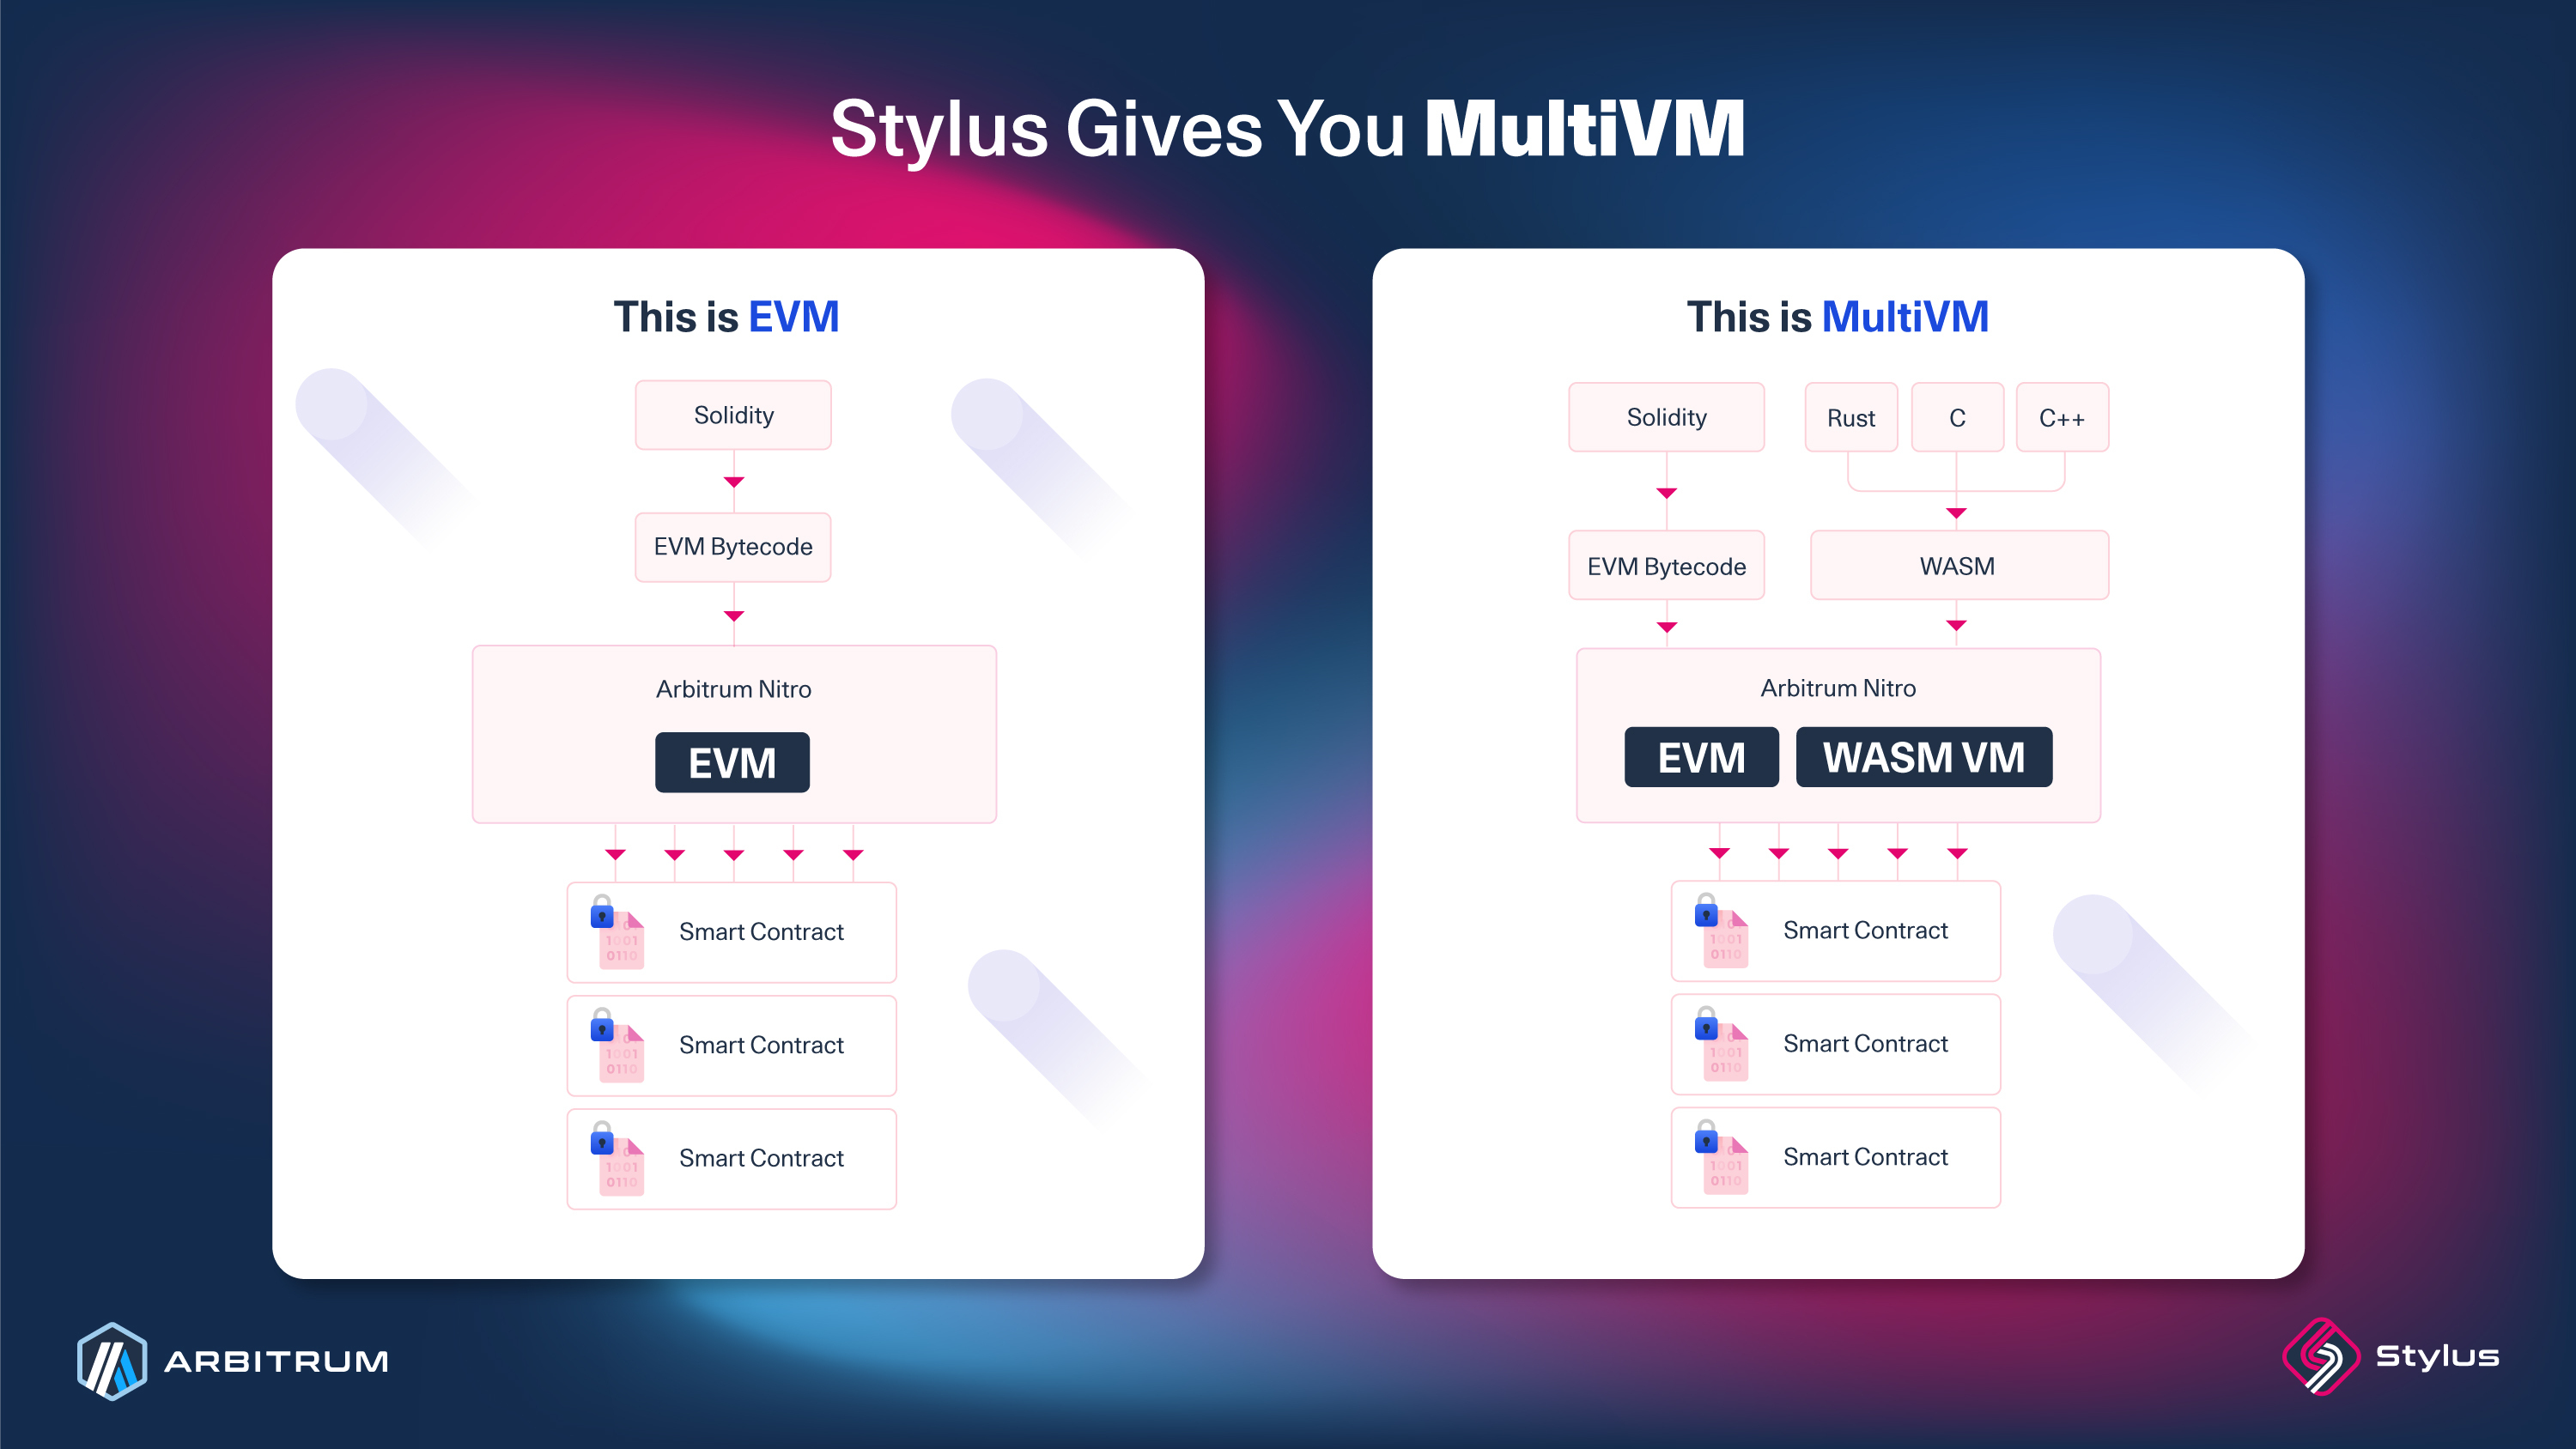
\includegraphics[width=0.70\textwidth]{general-problems/assets/arbitrum-nitro.png}
    \caption{Arbitrum Nitro}
    \label{fig:arbitrum-nitro}
\end{wrapfigure}

\subsubsection{R55-Eth}
